% Intersection of
% Author: Rasmus Pank Roulund
\documentclass{minimal}
\usepackage{tikz}
\usetikzlibrary{arrows}

\begin{document}
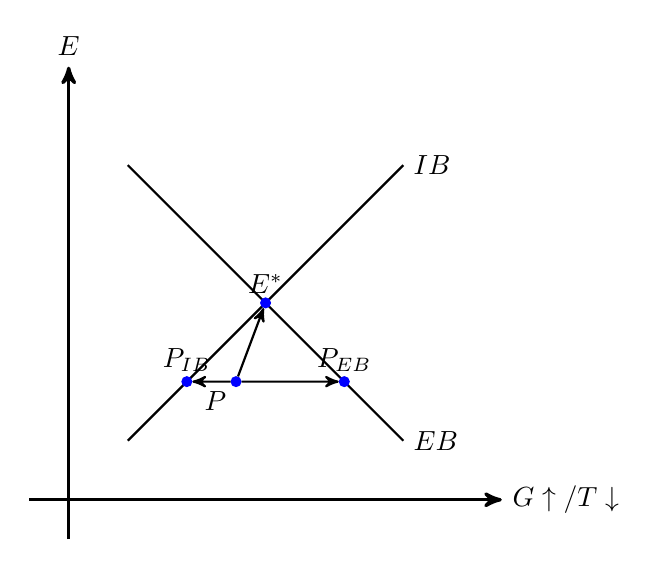
\begin{tikzpicture}[
    scale=5,
    axis/.style={very thick, ->, >=stealth'},
    important line/.style={thick},
    dashed line/.style={dashed, thin},
    pile/.style={thick, ->, >=stealth', shorten <=2pt, shorten >=2pt},
    every node/.style={color=black}
    ]
    % axis
    \draw[axis] (-0.1,0)  -- (1.1,0) node(xline)[right]
        {$G\uparrow/T\downarrow$};
    \draw[axis] (0,-0.1) -- (0,1.1) node(yline)[above] {$E$};

    % Lines
    % Modified label: Internal Balance (IB) instead of Y^O
    \draw[important line] (.15,.15) coordinate (A) -- (.85,.85)
        coordinate (B) node[right, text width=5em] {$IB$};
        
    % Modified label: External Balance (EB) instead of NX=x
    \draw[important line] (.15,.85) coordinate (C) -- (.85,.15)
        coordinate (D) node[right, text width=5em] {$EB$};

    % Intersection of lines
    % Modified color: blue
    % Modified label: E* (Equilibrium) instead of A
    \fill[blue] (intersection cs:
       first line={(A) -- (B)},
       second line={(C) -- (D)}) coordinate (E) circle (.4pt)
       node[above,] {$E^*$};

    % The E point is placed more or less randomly
    % Modified color: blue
    % Modified label: P (Point/Position) instead of B
    \fill[blue]  (E) +(-.075cm,-.2cm) coordinate (out) circle (.4pt)
        node[below left] {$P$};

    % Line connecting out and ext balances
    \draw [pile] (out) -- (intersection of A--B and out--[shift={(0:1pt)}]out)
        coordinate (extbal);
    % Modified color: blue
    % Modified label: P_IB (Point on Internal Balance) instead of C
    \fill[blue] (extbal) circle (.4pt) node[above] {$P_{IB}$};

    % line connecting  out and int balances
    \draw [pile] (out) -- (intersection of C--D and out--[shift={(0:1pt)}]out)
        coordinate (intbal);
    % Modified color: blue
    % Modified label: P_EB (Point on External Balance) instead of D
    \fill[blue] (intbal) circle (.4pt) node[above] {$P_{EB}$};

    % line between out og all balanced out :)
    \draw[pile] (out) -- (E);
\end{tikzpicture}
\end{document}
%%% Local Variables:
%%% mode: latex
%%% TeX-master: t
%%% End: